\chapter{Lab 3: Sequential Programming} \label{day3}



\section{Timer}

In this exercise one of the most useful and important tools of the \gls{fpga} gets used: the clock. This enables sequential programming which can be used to create sounds and much more as we will see in later exercises.

This module uses the 100\,Mhz clock of the \gls{fpga} and converts it into a lower frequency. Therefore the clock first needs to be enabled in the constraints file. This module uses a counter to create a slower clock. This method is not exactly precise as the counter cannot count in rational numbers, but its fairly close and sufficient for most use cases. For frequencies much lower than the input clock this module can be assumed to be accurate.

\lstinputlisting[language=VHDL]{./L3/E1/src/project_3_1.vhd}

\lstinputlisting[language=VHDL]{./L3/E1/src/project_3_1_1.vhd}

\lstinputlisting[language=VHDL]{./L3/E1/src/Constraints_all.xdc}

\section{Instantiating a netlist file}

In this exercise we use a given netlist file and instantiate it in our project to display a binary number on the four digit seven-segment display of the \gls{fpga}. 

\lstinputlisting[language=VHDL]{./L3/E2/src/project_3_2.vhd}

\section{Time counter}

Here, we programmed a counter that overflows implicitly and displays a new number every 0.5\,s on the four digit display of the \gls{fpga}. 

\begin{figure}[h]
	\centering
	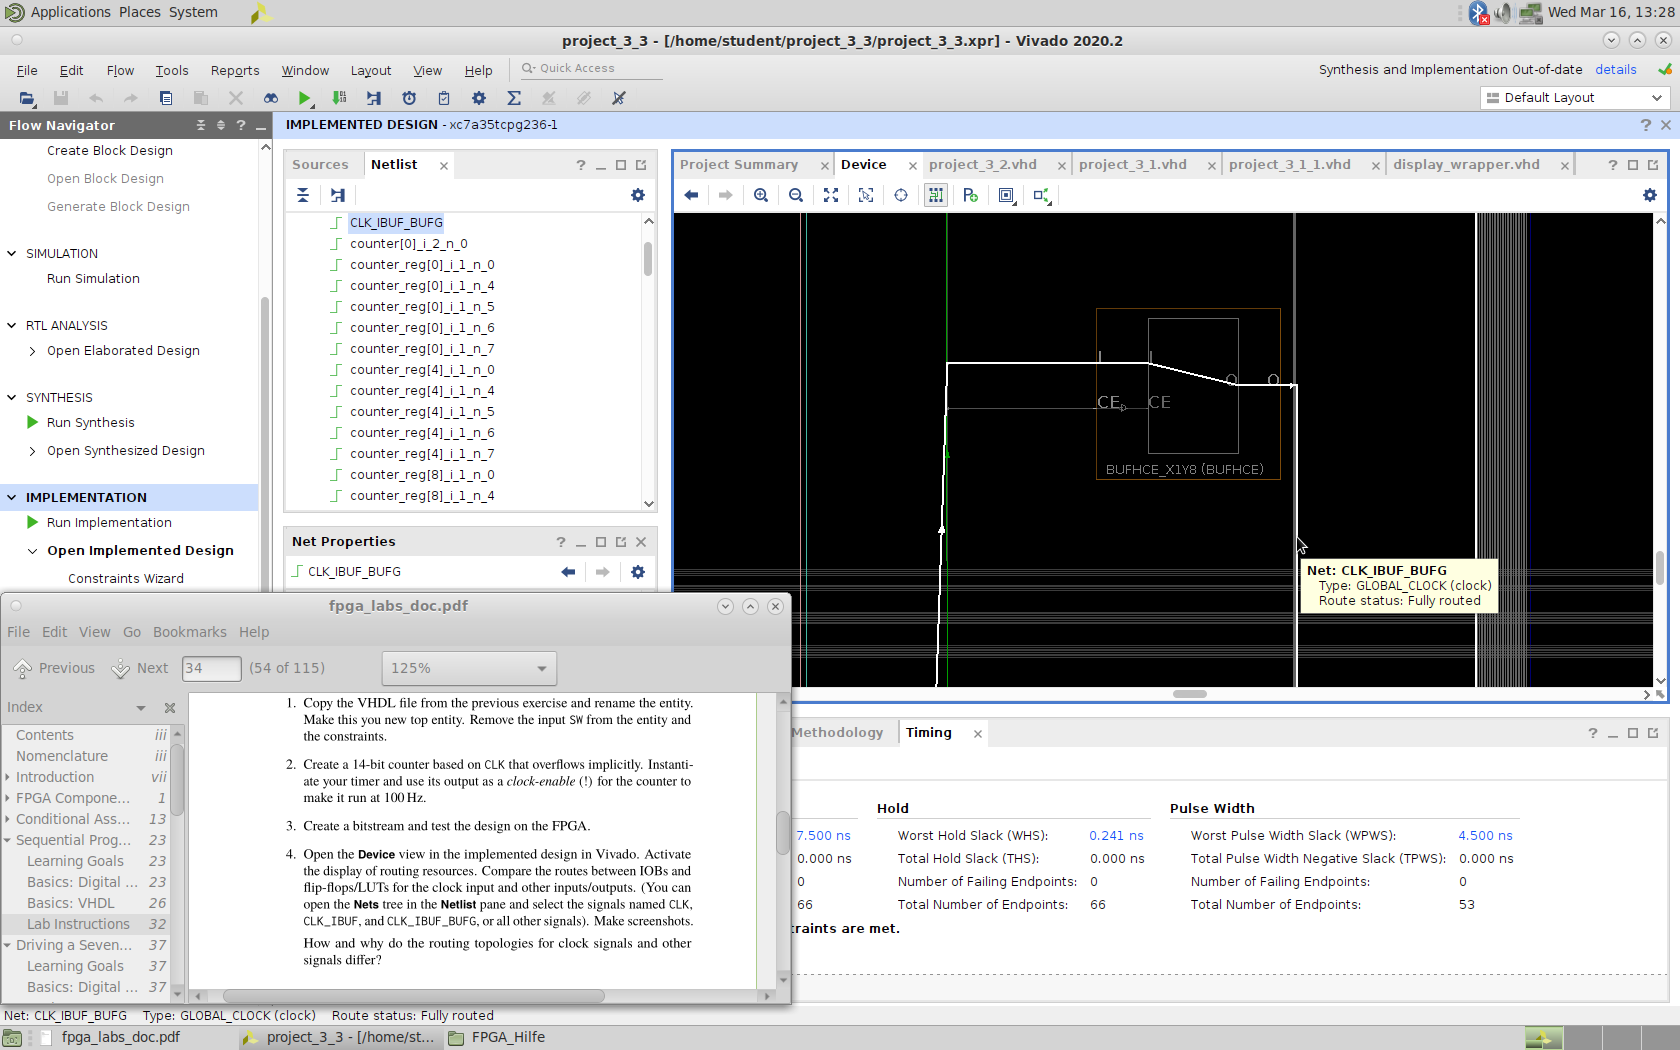
\includegraphics[width=.6\linewidth]{./L3/E3/BUFHCE.png}
	\caption{This clock signal is distributed via these centrally positioned buffer units on the \gls{fpga}.} 
	\label{fig: clock  e_3_3_1}
\end{figure}

\begin{figure}[h]
	\centering
	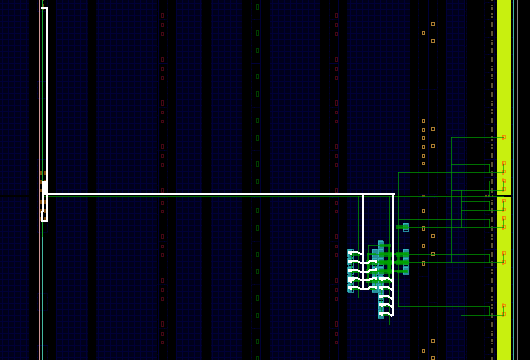
\includegraphics[width=.8\linewidth]{./L3/E3/CLK.png}
	\caption{The distribution of the clock signal. The clock signal is distributed over the central unit on the \gls{fpga} shown in fig. \ref*{fig: clock  e_3_3_1} and in this picture on the top left corner of the image. This design ensures that all the components of the circuit get almost the same clock signal to be in sync.}
	\label{fig: clock routing e_3_3_1}
\end{figure}

\lstinputlisting[language=VHDL]{./L3/E3/src/project_3_1_1.vhd}

\begin{figure}[h]
	\centering
	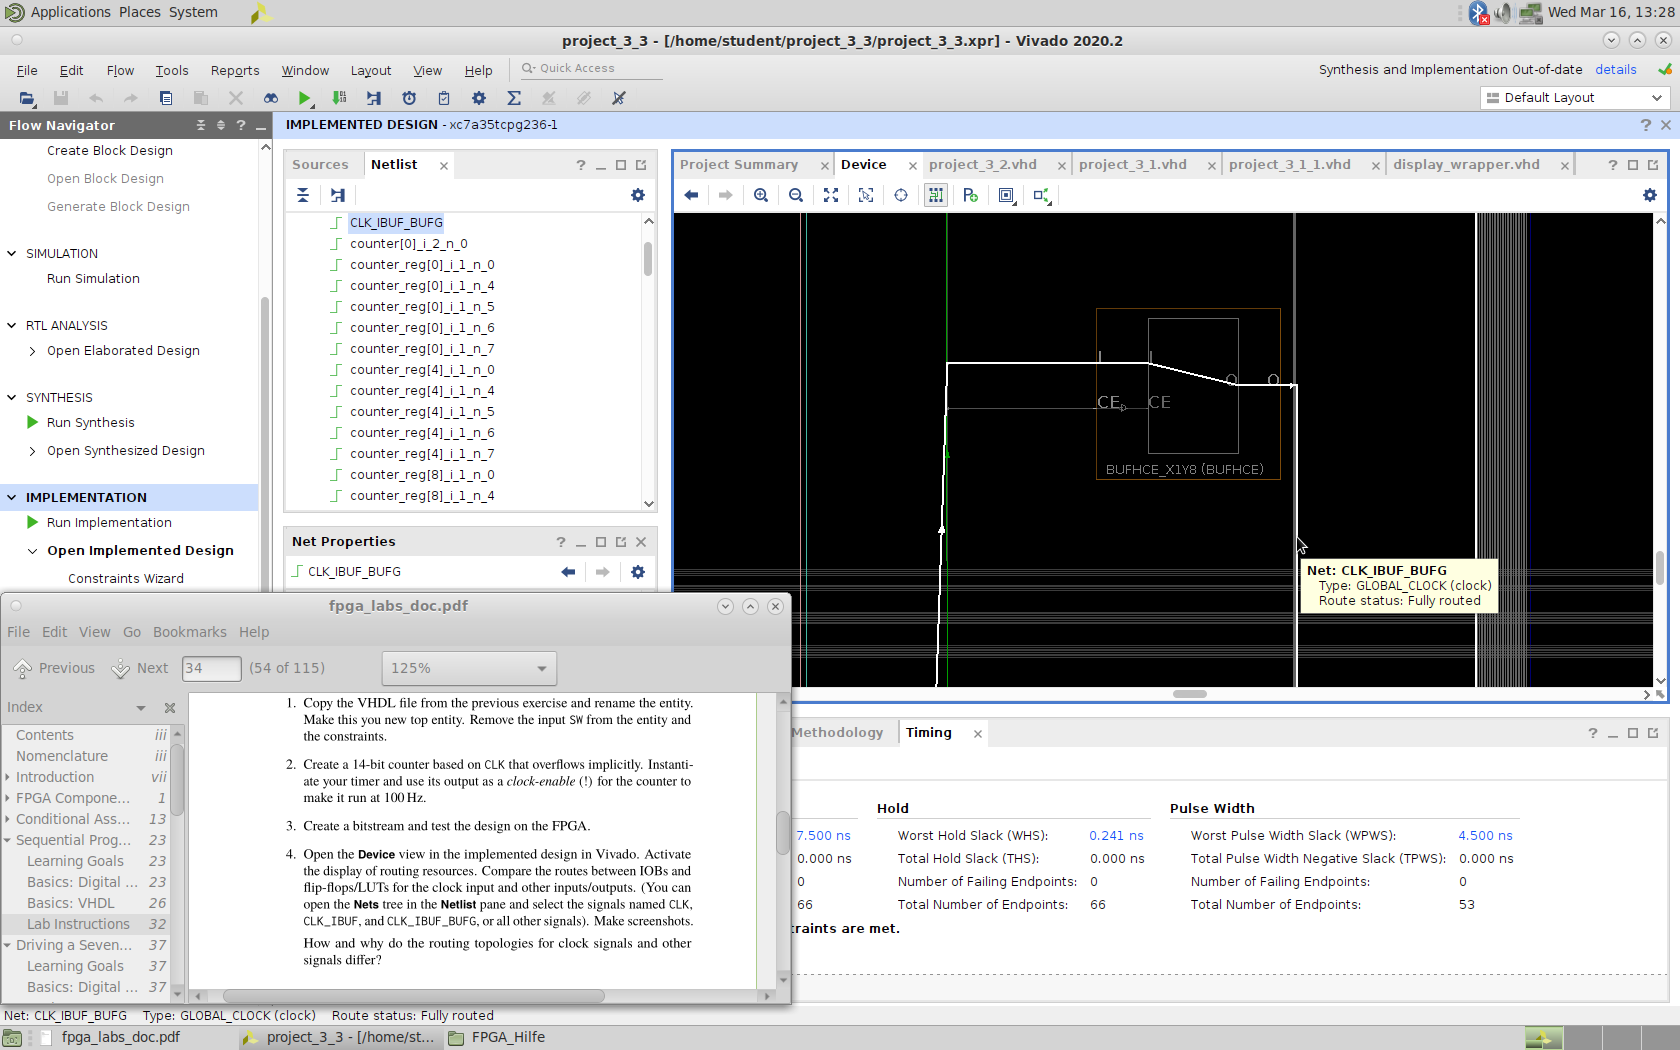
\includegraphics[width=.6\linewidth]{./L3/E3/BUFHCE.png}
	\caption{This clock signal is distributed via these centrally positioned buffer units on the \gls{fpga}.} 
	\label{fig: clock  e_3_3_1}
\end{figure}

\begin{figure}[h]
	\centering
	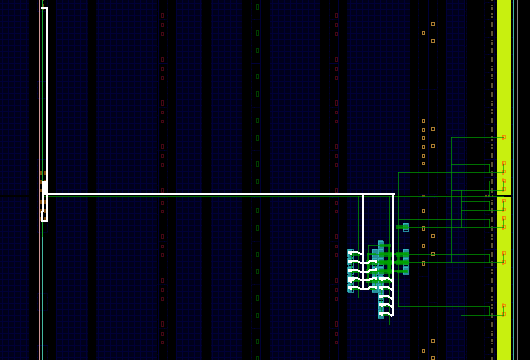
\includegraphics[width=.8\linewidth]{./L3/E3/CLK.png}
	\caption{The distribution of the clock signal. The clock signal is distributed over the central unit on the \gls{fpga} shown in fig. \ref*{fig: clock  e_3_3_1} and in this picture on the top left corner of the image. This design ensures that all the components of the circut get almost the same clock signal to be in sync.}
	\label{fig: clock routing e_3_3_1}
\end{figure}

%\lstinputlisting[language=VHDL]{./L3/E3/src/project_3_1_1.vhd}

%\lstinputlisting[language=VHDL]{./L3/E3/src/project_3_1.vhd}

\lstinputlisting[language=VHDL]{./L3/E3/src/project_3_3.vhd}

The clock signal differs from other signal due to the required equal distribution. Therefore the \gls{fpga} has multiple central distribution units that ensure exactly this as can be seen in fig. \ref{fig: clock routing e_3_3_1}. Otherwise sequential programming cannot work correcly as intended.

The clock signal differs from other signal due to the required equal distribution. Therefore the \gls{fpga} has multiple central distribution units that ensure exactly this as can be seen in fig. \ref{fig: clock routing e_3_3_1}. Otherwise sequential programming cannot work correctly as intended.

\section{Debouncing}

The integrated buttons on the board of the \gls{fpga} have to be debounced in order to be used as an input. As the button bounces up and down multiple times after being pressed only once the ``button-pressed''-status has to be checked with a much lower frequency than the 100\,MHz clock. When pressing the button 20 times and checking the status with the 100\,MHz clock we found that much more than 20 presses were counted. To fix the issue, we found that a 100\,Hz clock fits the job perfectly. Additionally we checked if the button has been pressed in the previous clock cycle of the 100\,Hz clock to eliminate any remaining errors. Checking the program with 50 button presses we found no errors.

\lstinputlisting[language=VHDL]{./L3/E4/src/edge_detector.vhd}

